\subsection{Server Sicherheitsmaßnahmen}


\subsubsection{Authentisierung und Autorisierung}



\subsubsection{Speichern von Anmeldedaten in der Datenbank\label{subsubsec:anmeldedaten_datenbank}}
Um die Skalierbarkeit der Anwendung zu gewährleisten, werden die Anmeldedaten der Benutzer in der Datenbank gespeichert.
Das hat den Vorteil, dass der Bezug zwischen Benutzer, Anmeldedaten und weiteren Informationen jederzeit gegeben ist, da keine externen Referenzen verwaltet werden müssen.
Ein Nachteil dieser Vorgehensweise ist jedoch, dass jeder Datenbankbenutzer mit Lesezugriff auf das \emph{hipsterbility}-Schema auf die Benutzerdaten zugreifen kann, wozu auch die Passwörter gehören.
Um diesen Nachteil zu relativieren nutzt der \emph{Glassfish 4} \ac{AS} standardmäßig die kryptografische Hashfunktion \emph{\ac{SHA}-2} mit 256~Bit Hashwerten (\ac{SHA}-256).

Zusätzlich zu der Speicherung der Hashwerte werden die Passwörter durch den Server mit der \emph{\ac{AES}} Blockchiffre verschlüsselt.
Als Passwort zur Ver- und Entschlüsselung wird das \emph{Glassfish} \texttt{Master Password} benutzt \cite[vgl.][16\psq]{OracleCorporation.2013}
Leider ist diese Funktion nur schlecht dokumentiert, es wird zwar grundlegend beschrieben wie ein \texttt{JDBCRealm} eingerichtet wird, jedoch nicht die Bedeutung der einzelnen Sicherheitsparameter \cite[vgl.][50\psq]{OracleCorporation.2013} nicht im Detail erläutert.

\subsection{Authentifizierung mit Java EE Security Realms}
Wie in Abschnitt \ref{subsubsec:anmeldedaten_datenbank} angedeutet, wird für die Verwaltung, Autorisierung und Authentifizierung der Serverkomponente ein \emph{JDBCRealm} eingerichtet.
\emph{Authentication Realms} bilden die Grundlage der Benutzersicherheitsmechanismen im \emph{Glassfish} \ac{AS} und ist Bestandteil von Java EE.
Zu den Hauptfunktionen gehört das Authentisieren, Identifizieren und Autorisieren.

Da für die Datenspeicherung ein \ac{DBMS} verwendet wird, bietet es sich an dort auch die Anmeldedaten der Benutzer zu speichern.

\subsubsection{JDBCRealm Datenbankschema und Entitätsklassen}
Das \texttt{JDBCRealm} sieht dazu ein Schema vor, welches mindestens aus zwei Tabellen besteht (siehe Abbildung \ref{fig:jdbcrealm_minimal_schema}), eine für die Benutzer und eine für Gruppen bzw. Rollen, welche von Benutzern eingenommen werden.
Die Namen der Tabellen und Spalten können bei der Konfiguration angegebene werden und sind entsprechend flexibel.
Benötigt werden eine Tabelle mit Benutzernamen und Passwort (\texttt{Users}) und eine mit der Zuordnung von Gruppenname und Benutzername (\texttt{Groups}).

Bei der Verwendung der \ac{JPA} könnten die zugehörigen Entity-Klassen beispielsweise aussehen, wie in Listings \ref{lst:jdbcrealm_klasse_benutzer} und \ref{lst:jdbcrealm_klasse_gruppe}.

\begin{minipage}[t]{0.5\textwidth}
\begin{lstlisting}[language=Java,caption={Beispiel für eine UserEntity Klasse.}, label=lst:jdbcrealm_klasse_benutzer]
// [...] Imports etc.
@Entity(name = "Users")
public class UserEntity {

    @Id
    private String username;
    private String password;
    // [...] Getter und Setter.
}
\end{lstlisting}
\end{minipage}
\begin{minipage}[t]{0.5\textwidth}
\begin{lstlisting}[language=Java,caption={Beispiel für eine GroupEntity Klasse.}, label=lst:jdbcrealm_klasse_gruppe]
// [...] Imports etc.
@Entity(name = "Groups")
public class GroupEntity {

    @Id
    private int id;
    private String name;

    @ManyToOne
    @JoinColumn(name = "username")
    private UserEntity user;
    // [...] Getter und Setter.
}
\end{lstlisting}
\end{minipage}

Dieses Schema hat allerdings, besonders bei der Verwendung der \ac{JPA} einige Nachteile.
Einerseits verhindert es das einfache Verwenden von numerischen Primärschlüsseln bei der Tabelle \texttt{Users}, da das \texttt{JDBCRealm} in der Gruppentabelle einen Benutzernamen und keine ID erwartet. 
Andererseits kann die selbe Gruppe einem Benutzer mehrfach zugeordnet werden, da keine Beschränkungen vorliegen.

\begin{minipage}[t]{\textwidth}
	\centering
	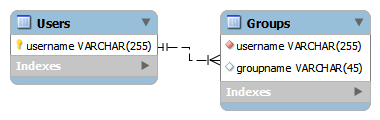
\includegraphics[scale = .75]{img/jdbcrealm_schema}
	\captionof{figure}{Beispielhaftes minimales Datenbankschema für ein JDBCRealm.}
	\label{fig:jdbcrealm_minimal_schema}
\end{minipage}

\subsubsection{Anpassungen bei der Realisierung}

Die Entitätsklassen und folglich auch das Datenbankschema wurde entsprechend der Nachteile angepasst.
Die Anpassungen sind in Listings \ref{lst:jdbcrealm_klasse_benutzer_code} und \ref{lst:jdbcrealm_klasse_gruppe_code} dargestellt.

Um die Verwendung von numerischen Benutzer--IDs zu ermöglichen wurde eine View erstellt, die das erwartete Schema abbildet, siehe Listing \ref{lst:jdbcrealm_view_code}.
Außerdem wurden entsprechende Beschränkungen in den Tabellen eingeführt.
\begin{lstlisting}[language=SQL,caption={SQL Befehl zum erstellen einer View mit Benutzername und Gruppenname}, label=lst:jdbcrealm_view_code]
CREATE VIEW usergroup AS SELECT u.USERNAME, g.NAME FROM USER u INNER JOIN realmgroup g on g.USER_ID = u.ID WHERE u.ACTIVE=1;
\end{lstlisting}
Die View hat weiterhin den Vorteil, dass die Auswahl nur aktive Benutzerkonten enthält.
Wenn das Feld \texttt{ACTIVE} in der Tabelle \texttt{user} den Wert \texttt{1} hat, wird der Benutzer gelistet, hat das Feld den Wert \texttt{0}, so wird er nicht in der Auswahl erfasst.
So lassen sich Benutzerkonten deaktivieren um die Anmeldung zu verhindern, müssen jedoch nicht aus der Datenbank entfernt werden.

Da der Benutzername nicht mehr der Primärschlüssel ist, wurde eine Beschränkung eingeführt, um den Benutzernamen in der Tabelle eindeutig zu halten.
Außerdem darf er, nach dem Erstellen, nicht mehr geändert werden und muss einen Wert enthalten.
\begin{lstlisting}[language=Java,caption={Beispiel für eine UserEntity Klasse.}, label=lst:jdbcrealm_klasse_benutzer_code]
// [...] Imports etc.
@Entity(name = "User")
// [...]
public class UserEntity {
	// [...]
    @Id
    @GeneratedValue(strategy= GenerationType.IDENTITY)
    private int id;
    @Column(unique = true, nullable = false, updatable = false)
    private String username;
    // [...]
    @Column(nullable = false) @XmlTransient @JsonIgnore
    private String password;
    // [...] Getter, Setter und weitere Properties.
\end{lstlisting}

Die Gruppen oder Rollentabelle wurde um Beschränkungen erweitert, die eine Mehrfachzuordnung des selben Benutzers zu einer einzigen Gruppe untersagen.
\begin{lstlisting}[language=Java,caption={Auszug aus der GroupEntity Klasse.}, label=lst:jdbcrealm_klasse_gruppe_code]
// [...] Imports etc.
@Entity(name = "RealmGroup")
@Table(uniqueConstraints = @UniqueConstraint(columnNames = {"NAME, USER_ID"}))
public class GroupEntity {
    // [...]
    @Id
    @GeneratedValue(strategy=GenerationType.IDENTITY)
    private int id;
    @Column(nullable=false)
    private String name;
    @ManyToOne
    private UserEntity user;
    // [...] Getter und Setter.
}
\end{lstlisting}

Wenn die nötigen \ac{JDBC}"~Ressourcen bereits erstellt wurde, kann das \texttt{JDBCRealm} mit dem Befehl aus Listing \ref{lst:asadmin_create_realm} mit dem \texttt{asadmin}"~Werkzeug erzeugt werden.
Das Erstellen und Bearbeiten von Realms ist auch über die Weboberfläche möglich, siehe Abbildung \ref{fig:realm_screenshot}.


